\documentclass[12pt]{beamer}

\usepackage{cmap}
\usepackage[T2A]{fontenc}
\usepackage[utf8]{inputenc}
\usepackage[russian]{babel}
\usepackage{amsthm, amsmath, amssymb}
\usepackage{hyperref}
\usepackage{datetime}
\usepackage{cmap}
\usepackage{enumerate}
\usepackage{color}
\usepackage{picture}
\usepackage{graphicx}
\usepackage{tikz}
\usepackage{xcolor}
\usetikzlibrary{positioning,shadows,arrows}

\usepackage{bold-extra}

\def\EPS{\varepsilon}
\def\SO{\Rightarrow}
\def\EQ{\Leftrightarrow}
\def\t{\texttt}

\usetheme{Luebeck}
\usecolortheme{beaver}

\let\Tiny=\tiny
\useoutertheme{infolines}

\tikzset {
    fact/.style={rectangle, draw=none, rounded corners=1mm, fill=blue, drop shadow,
        text centered, anchor=north, text=white},
    new/.style={circle, draw=none, fill=orange, circular drop shadow,
        text centered, anchor=north, text=white},
    state/.style={circle, draw=none, fill=red, circular drop shadow,
        text centered, anchor=north, text=white},
    leaf/.style={rectangle, draw=black,
    minimum width=0.5em, minimum height=0.5em},
    cur/.style={circle, draw=none, fill=green, circular drop shadow,
        text centered, anchor=north, text=black},
    level distance=1.0cm, anchor=south
}

\begin{document}

\title{Blackout}

\author[]{
    Andrei Tonkikh \\
    Nikita Sazanovich \\
}
\institute[]{Saint Petersburg Academic University}
\date{February 27, 2017}

\frame{\titlepage}


\begin{frame}{Project idea}
    \begin{itemize}
        \item <1-> Dynamic multiplayer action-arena game with RPG elements and a rich system of spell interactions.
	      \item <2-> Social features: ratings, achievements, leaderboard.
        \item[] <3-> \begin{center} 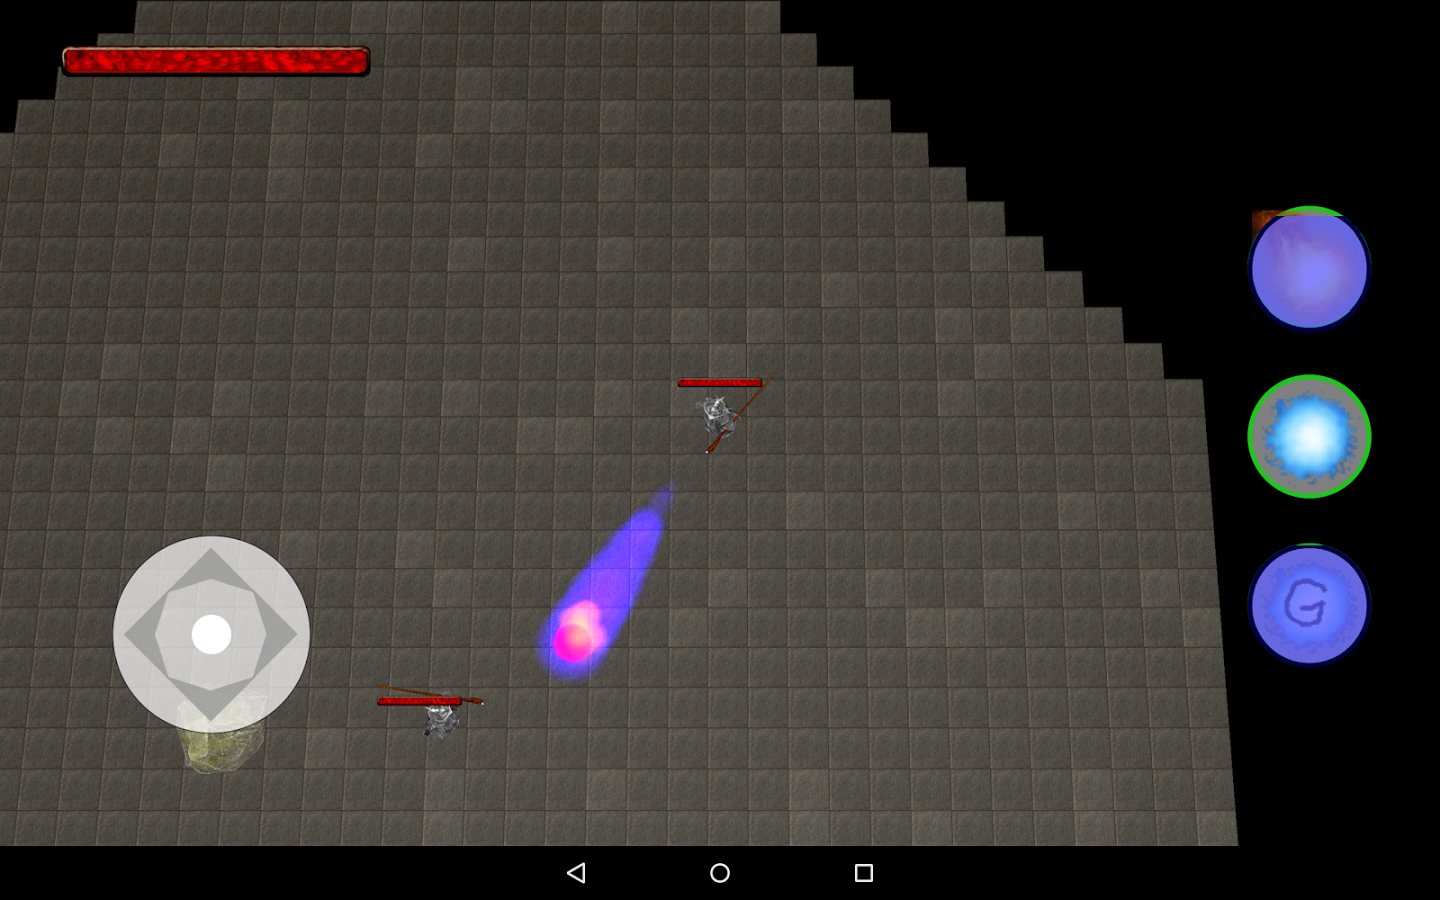
\includegraphics[width=230pt]{screenshot.png} \end{center}
    \end{itemize}
\end{frame}


\begin{frame} {Technologies}
    \begin{itemize}
        \item Game engine: libGDX.
        \item Physics engine: Box2D.
        \item Other tools: Git, Travis CI, Blender, GIMP, Inkscape...
    \end{itemize}
\end{frame}



\begin{frame} {Architecture}
\noindent\makebox[\textwidth]{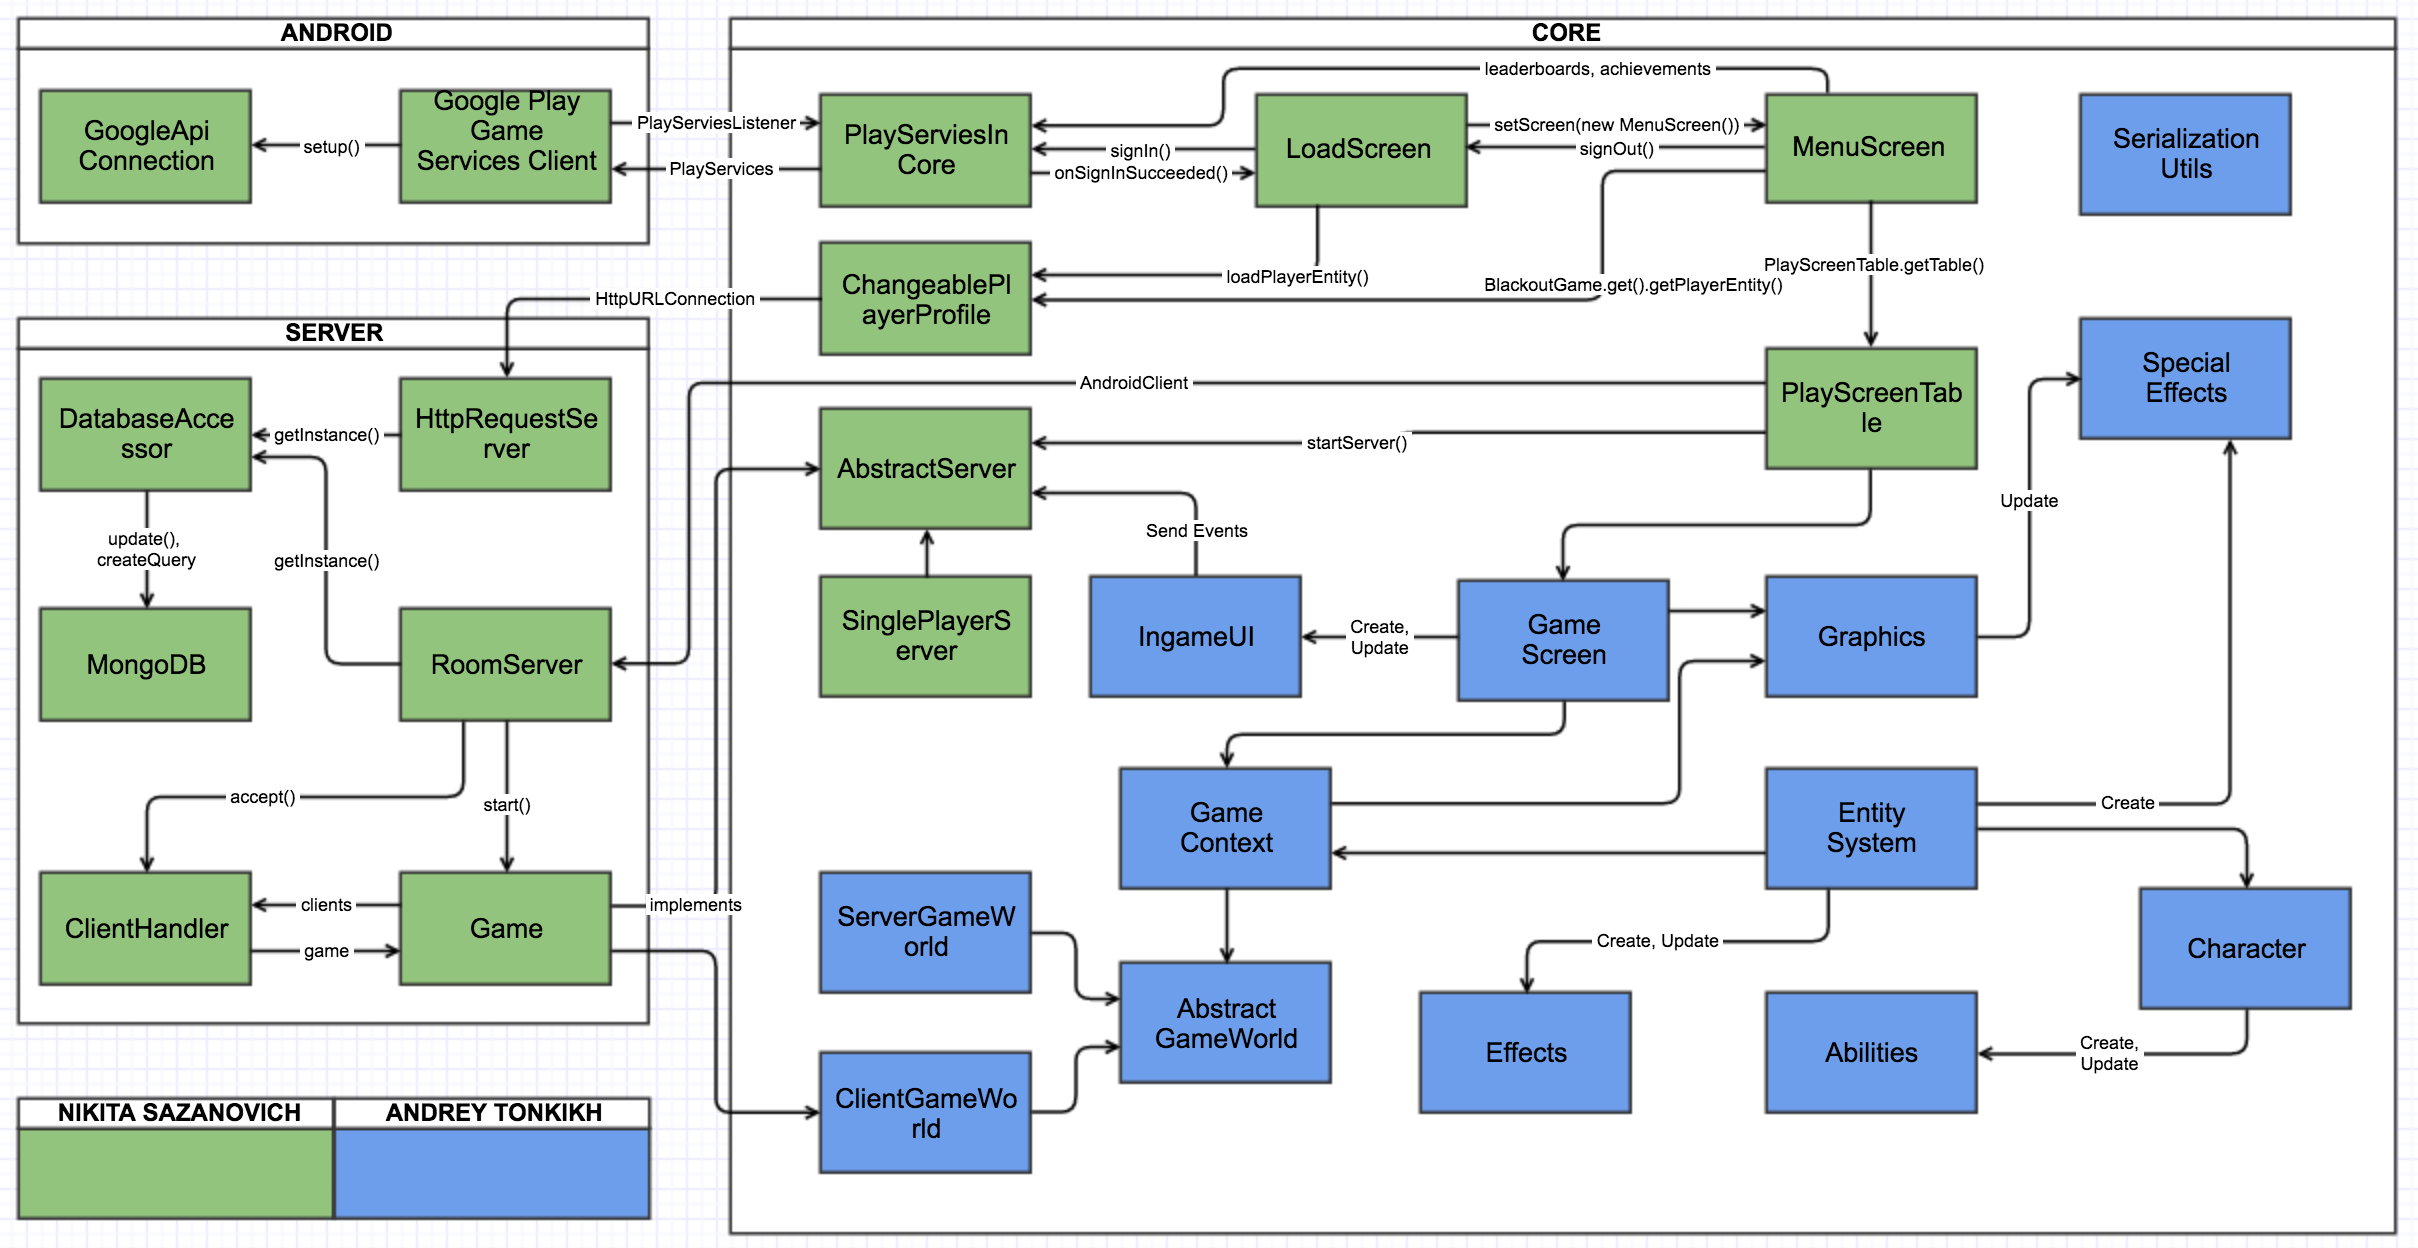
\includegraphics[width=\paperwidth]{architecture.png}}
\end{frame}


\begin{frame} {Android and Server}
    \begin{itemize}
        \item <1-> Integration with Google Play Games Services.
        \item <2-> Game UI made with libGDX.
        \item <3-> Which database to use -- Saved Games (Google Drive) or local DB (MongoDB)?
        \item <4-> Server choices: for user requests -- HttpServer, for in-game synchronization -- Java Sockets.
        \item <5-> Game servers are local.
    \end{itemize}
\end{frame}


\begin{frame} {Synchronization problems}
    \begin{itemize}
    	\item <1-> Which synchronization model to choose: peer-to-peer (Google Play Game Services), one of the players is a server or client-server?
	    \item <2-> Should we calculate any physics on the client or always get the world from the server?
	    \item <3-> Network options reasearch: TCP$\rightarrow$UDP, custom serialization
    \end{itemize}
\end{frame}


\begin{frame} {Abstracting from single and multi player modes}
    \begin{itemize}
        \item[] <1-> Aimed for reusing the same classes for single and multi player modes.
        \item[] <2-> \begin{center} 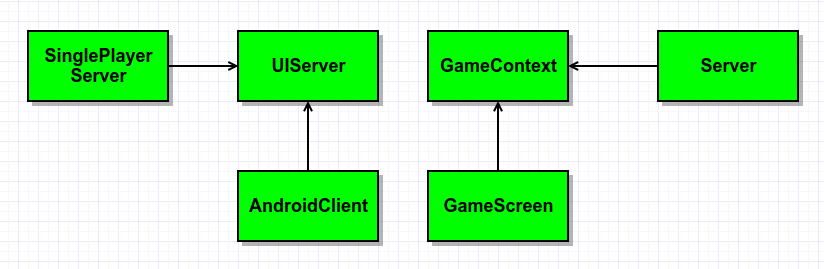
\includegraphics[width=300pt]{singleplayer.png} \end{center}
    \end{itemize}
\end{frame}


\begin{frame}{Graphics and other resources}
    \begin{itemize}
        \item <1-> Models are taken from: http://opengameart.org/
        \item <2-> 2D $\rightarrow$ 3D
        \item <3-> Blender, Inkscape, GIMP
        \item <4-> Particle effects
    \end{itemize}
\end{frame}


\begin{frame}{Changelog}
    \begin{itemize}
        \item New spell: Gravity.
        \item By using custom serialization and compressing the data, decreased the network traffic by 75-80\%.
        \item Introduced rating system.
        \item Dynamic improvements' cost system.
    \end{itemize}
\end{frame}


\begin{frame}{Futher improvements}
    \begin{itemize}
        \item <1-> Make competitive AI
        \item <2-> Introduce new game content: game modes, spells...
        \item <3-> More complex improvements' cost system, players' experience levels
        \item <4-> More social features, like duels...
    \end{itemize}
\end{frame}


\begin{frame}{Results}
    \begin{itemize}
        \item Google play open alpha testing: \\ https://play.google.com/apps/testing/ru.spbau.blackout.android
        \item Github: \\
        https://github.com/niksaz/blackout
        \item Demo video: \\
        https://www.youtube.com/watch?v=0VuFQBdPXMM
    \end{itemize}

\end{frame}


\end{document}
